\documentclass{elsarticle}
%\usepackage[pdftex,breaklinks,linktocpage,pagebackref,hyperindex,hyperfigures]
\usepackage{hyperref}
\usepackage[utf8]{inputenc}
\usepackage{amsmath}
\usepackage{amsthm}
\usepackage{amssymb}
\usepackage[tmargin=1in,bmargin=1in]{geometry}
\usepackage{subfigure}
\usepackage{graphicx}
\usepackage{latexsym}
\usepackage{pdfsync}
\usepackage[boxed]{algorithm}
\usepackage{algpseudocode}
\usepackage{algorithm}
%\usepackage{algorithmic}
\usepackage{multirow}
\usepackage{rotating}
\usepackage{color}
\usepackage{caption}
\usepackage{url}

\hypersetup{
    colorlinks=true,      		% false: boxed links; true: colored links
    linkcolor=blue,       		% color of internal links
    citecolor=blue,       		% color of links to bibliography
    filecolor=black,      		% color of file links
    urlcolor=red,       		% color of external links
    bookmarks=false,
    pdffitwindow=true,
    pdfpagelayout=SinglePage
}

\newcommand{\etal}{\textit{et al.\ }}
\newcommand{\pd}[2]{\frac{\partial #1}{\partial #2}}
\newcommand{\mbf}[1]{\mathbf{#1}}
\newcommand{\comment}[1]{\textcolor{red}{#1}}
\newcommand{\tensor}[1]{\underline{\underline{\boldsymbol{#1}}}}

\newtheorem{property}{Property}


\begin{document}

\begin{frontmatter}
\title{Level-Set method on \texttt{p4est}}

\cortext[cor]{Corresponding author: arthur.guittet@gmail.com}

\address[MECHE]{Department of Mechanical Engineering, University of California, Santa Barbara, CA 93106-5070}
\address[CS]{Department of Computer Science, University of California, Santa Barbara, CA 93106-5110}

 \author[MECHE]{Mohammad Mirzadeh} \author[MECHE]{Arthur Guittet} \author[MECHE,CS]{Fr\'ed\'eric Gibou}

\begin{abstract}
cool abstract
\end{abstract}
\begin{keyword}
p4est \sep Level-Set
\end{keyword}

\end{frontmatter}

\section{Introduction}

\section{The level-set method}

\indent The level-set method is a method to capture interfaces implicitely by constructing a function $\phi$, called the level-set function, that is negative on on side of the domain $\Omega^-$ and positive on the other side $\Omega^+$, thus defining the interface $\Gamma$ as the zero contour of $\phi$, $\Gamma = \{\mathbf{x} \vert \phi(\mathbf{x}=0\}$.\\

If infinitely many functions satisfy these requirements, the most natural and most convenient representation is a signed distance function to the interface. The level-set function is therefore reinitialized to a signed distance function at every time step by solving the reinitialization equation

\begin{equation} \label{eq::reinitialization}
\pd{\phi}{\tau} + \mathrm{sign}(\phi) \left( \lvert \phi \rvert - 1 \right) = 0,
\end{equation}

where $\tau$ is a fictitious time. The discretization and implementation of this procedure will be discussed later in section \ref{section::reinitialization}. Geometrical quantities such as the normal to the interface and the local curvature can be computed straightforwardly from the level-set function as

\begin{equation*}
\mathbf{n} = \frac{\nabla \phi}{\lvert \nabla \phi \rvert},
\end{equation*}

where it should be noted that $\lvert \nabla \phi \rvert = 1$ when the level-set function is reinitialized, and

\begin{equation*}
\kappa = \nabla \cdot \mathbf{n} =  \nabla \cdot \left( \frac{\nabla \phi}{\lvert \nabla \phi \rvert} \right).
\end{equation*}


\section{The \texttt{p4est} library}

The work we present relies on the parallel octree library \texttt{p4est} \cite{burstedded:2011:p4est}. It is scalable implementation of the general octree structure in a massively parallel mpi environment. We limit our presentation of \texttt{p4est} to the relevant information for our application, for more details the reader is invited to read the original article \cite{burstedded:2011:p4est}.

The \texttt{p4est} library provides the geometrical information for the leaves of an octree which includes the neighboring information for the leaves (called quadrants in the original article) of the tree, a layer of ghost quadrants and ghost vertices for each process, the coarsening and refining procedures, and encapsulates the communication between processes. However, it does not provide the vertical structure of the octrees. If it is generally unnecessary, it is a desirable feature for a finite differences based code as it speeds up the access to arbitrary quadrants information dramatically. Thus, we choose to reconstruct the local vertical structure of the octree on every processes. Note that given the local and ghost layer information, this is an entirely local procedure and no communication is needed.

In addition to the owned and ghost categories, we choose to group the vertices in \textit{local} and \textit{layer} sets. We define the layer vertices as the vertices that are part of another process's ghost layer and the local vertices as the vertices that are not part of any other process's ghost layer. Figure \ref{fig::local_layer_vertices} gives a graphical representation of a boundary between two processes and the classification of the various quadrants and vertices. The idea behind this sorting is that layer vertices are needed by other processes for finite difference calculations and therefore require to be synchronized while the local vertices are used only by the process they belong to. We make use of this classification to implement scalable algorithms for the level-set method, as explained in the following sections.

\begin{figure}[ht!]
\begin{center}
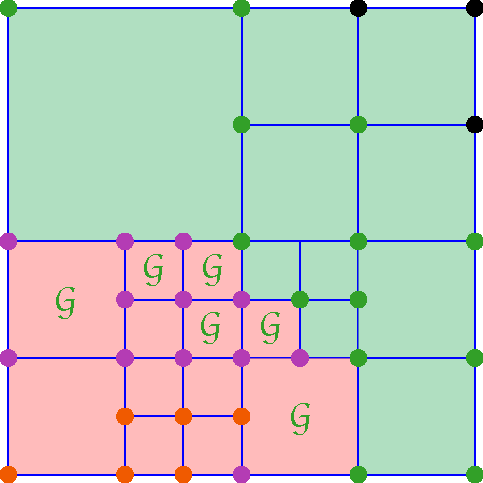
\includegraphics[width=.4\textwidth]{pictures/layer_nodes.pdf}
\caption{Illustration of a possible layout at the interface between two processes. The red quarants and the orange and purples vertices belong to process 1 while the green quadrants and the green and black vertices belong to process 2. The green G denotes the ghost quadrants for process 2, the green dots are the ghost vertices for process 1, and the purple dots correspond to layer vertices for process 1 (and therefore ghost vertices for process 2).} \label{fig::local_layer_vertices}
\end{center}
\end{figure}

\section{Presentation of the algorithms}

We now propose a detailed description of the main algorithms for the level-set method.

\subsection{Interpolations}

The first important step to build a level-set based code is to provide an interpolation procedure on the vertices. Being able to evaluate quantities at arbitrary locations in the computational domain is mandatory for procedures such as advecting the level-set function or enforcing boundary conditions on the irregular interface. The interpolation procedure enables any process to evaluate a quantity anywhere in the domain.

\begin{algorithm}[ht!]
\begin{algorithmic}
\If {interpolation order $>$ 2}
	\State compute second order derivatives for local and ghost points if needed
\EndIf
\State begin send point buffer
\State do the interpolation for local points
\State do the interpolation for ghost points
\State begin receiving point buffer
\For {in $\in$ \{remote senders\} }
	\State finish receiving from send i
	\State interpolate all points from sender i
\EndFor
\State receive the point buffer
\end{algorithmic}
\end{algorithm}

\subsection{Semi lagrangian advection}

\subsection{Reinitialization and extensions} \label{section::reinitialization}

The reinitialization procedure transforms an arbitrary function into a signed distance function to its zero contour. One of the popular methods to achieve this results is to solve the reinitialization equation \ref{eq::reinitialization} \cite{Sussman:1994:levelsetincompressible, Min_Gibou:2007:Level_Set_Adaptive}. Other methods, such as the Fast Sweeping \cite{??} and the Fast Marching methods \cite{Sethian:1996:FMM, chopp:2001:fmm}, are based on the wave propagation nature of the reinitialization front and provide faster implementations of the reinitialization procedure in a serial environment. However, their parallelization is an involved process and we opt for solving the reinitialization equation.

We base our approach on Min and Gibou \cite{Min_Gibou:2007:Level_Set_Adaptive} and discretize the reinitialization equation as

\begin{equation*}
\frac{d\phi}{d\tau} + \mathrm{sign}(\phi^0)[H_G(D^+_x\phi, D^-_x\phi, D^+_y\phi, D^-_y\phi)-1] = 0,
\end{equation*}

with $\mathrm{sign}(\phi^0)$ the signum of the initial level-set function and $H_G$ the Godunov Hamiltonian:

\begin{equation*}
H_G(a,b,c,d) =
\begin{cases}
\sqrt{\max(\lvert a^+ \rvert^2, \lvert b^- \rvert^2) + \max(\lvert c^+ \rvert^2, \lvert d^- \rvert^2)} \quad \mathrm{if~sgn}(\phi^0) \leq 0\\
\sqrt{\max(\lvert a^- \rvert^2, \lvert b^+ \rvert^2) + \max(\lvert c^- \rvert^2, \lvert d^+ \rvert^2)} \quad \mathrm{if~sgn}(\phi^0) > 0
\end{cases}
\end{equation*}

with $a^+=\max(a,0)$ and $a^-=\min(a,0)$. The one-sided derivatives $D^{+/-}_{x/y}\phi$ are discretized by second order accurate finite differences as explained by Min and Gibou in \cite{Min_Gibou:2007:Level_Set_Adaptive}. Following the presentation in \cite{Min_Gibou:2007:Level_Set_Adaptive} which incorporates the subcell resolution introduced by Russo and Smereka \cite{Russo_Smereka}, we include the initial position of the interface, given by $\phi^0$, in the computation of the one sided derivatives next to the interface in order to preserve the interface location. Finally, we choose a simple Euler step for the time discretization.

The general parallel algorithm for the reinitialization procedure is presented in \ref{algo::reinitialization}. For each fictitious time step, we start by computing the new value of the level-set function for the layer nodes. We then initiate the communication to update the ghost values while computing the new values for local nodes. After finishing the communication, we can then update $\phi^n$ to $\phi^{n+1}$ and move on to the next time step. The number of iterations needed for the reinitialization procedure to converge on the whole domain or on a band surrounding the interface depends on the size of the mesh, the geometry of the interface and how far from a signed distance function $\phi^0$ is. In practice, twenty iterations provide reasonable results for the applications we present.

\begin{algorithm}[ht!]
\begin{algorithmic}
\State Compute initial derivatives of $\phi$ for subcell resolution
\For {number of iterations}
	\State Compute the derivatives of $\phi$
	\State Solve reinitialization of layer nodes: $\phi_{layer} \leftarrow \phi_{layer}^{n+1}$
	\State Begin update for layer nodes
	\State Solve reinitialization on local nodes : $\phi_{local} \leftarrow \phi_{local}^{n+1}$
	\State End update for layer nodes
	\State Update $\phi$: $\phi \leftarrow \phi^{n+1}$
\EndFor
\end{algorithmic}
\caption{General structure of the parallel implementation of the reinitialization procedure presented in section \ref{section::reinitialization}.} \label{algo::reinitialization}
\end{algorithm}

\section{scalability and accuracy}

\subsection{Interpolation}

\begin{figure}[ht!]
\begin{center}
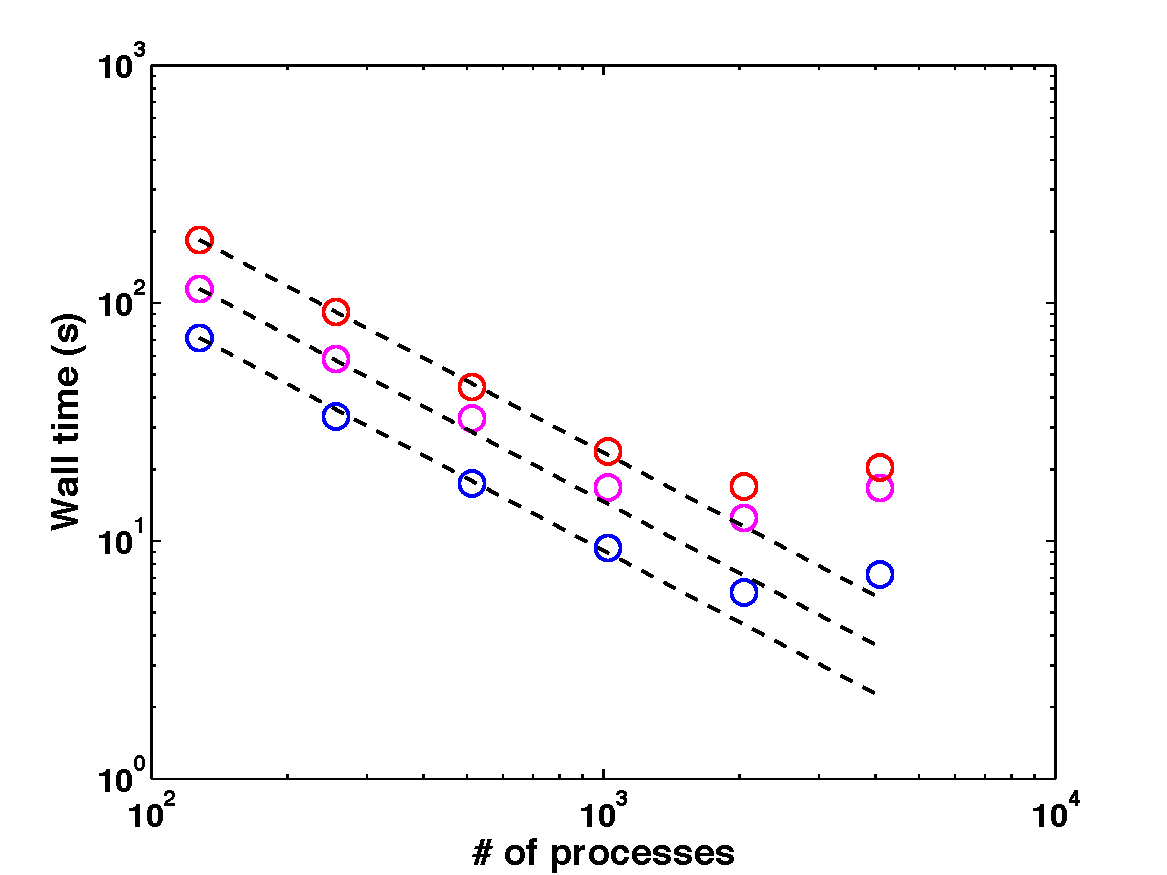
\includegraphics[width=.7\textwidth]{pictures/scaling_interpolation_all.pdf}
\caption{Scalability of the interpolation procedure. blue: alpha=0.05, purple alpha=0.50, red alpha=0.95 (alpha = percent of non-local points)}
\end{center}
\end{figure}


\subsection{Semi lagrangian advection}

\subsection{Reinitialization} \label{section::scaling_reinitialization}

The reinitialization procedure presented in section \ref{section::reinitialization} necessitates the second order derivatives of the level-set function for the second order discretization in space. The finite difference schemes we implemented rely on the description of the neighborhood of each vertex in the adaptive tree environment. This information can either be computed on the fly or stored in a buffer. Fetching the neighbors information is rather time consuming and was observed to improve the overall scalability of the algorithm by increasing the local computation load. However, it slowed down the procedure significantly and therefore we choose to present the buffered version of the implementation. If one was to be limited in memory, constructing the neighborhood information on the fly would be a desirable option and would lead to better scaling, but in our case memory is not a limiting factor.

The scaling results are presented in figure \ref{fig::scaling_reinitialization} and demonstrate satisfying scalability. Taking for reference the timing with $128$ processes, we observe efficiencies of $0.877$ with $1024$ processes, $0.763$ with $2048$ processes and $0.609$ with $4096$ processes.

\begin{figure}[ht!]
\begin{center}
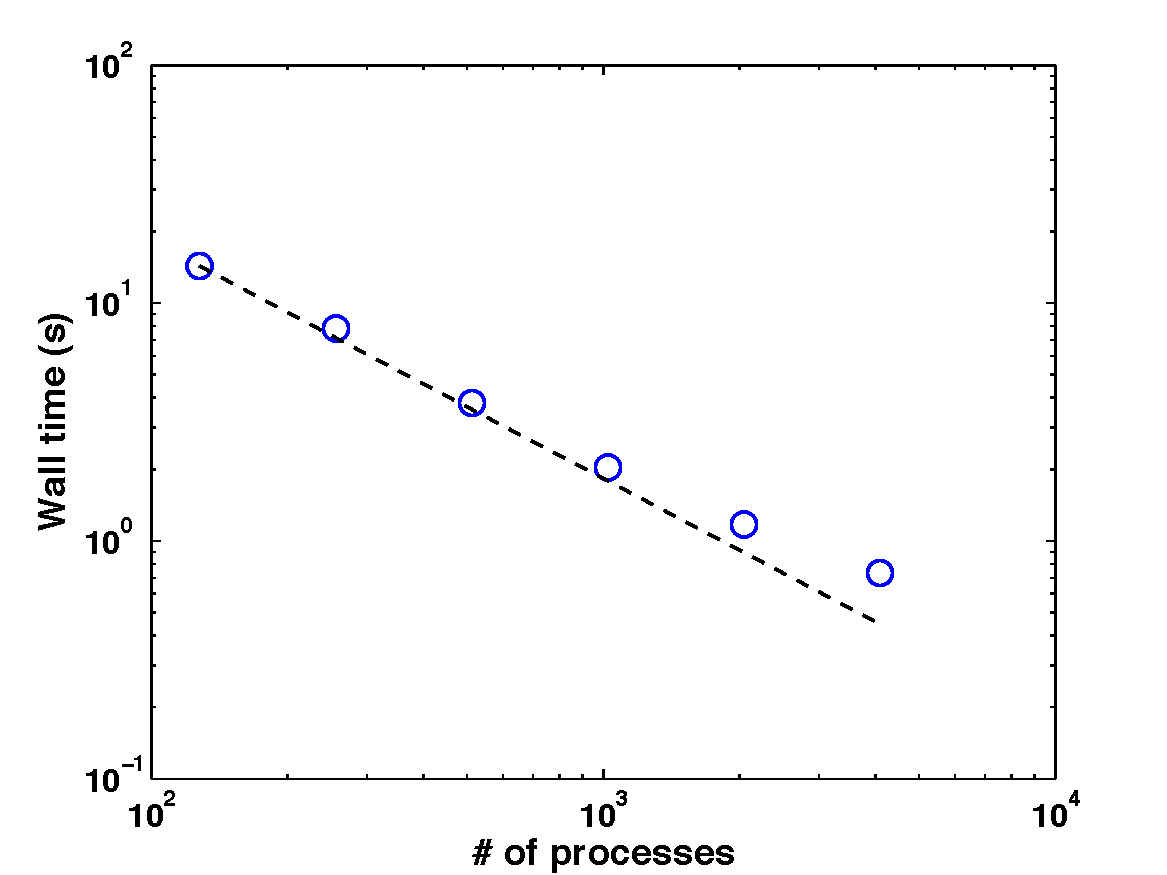
\includegraphics[width=.7\textwidth]{pictures/scaling_reinitialization_1st_time_2nd_space_with_buffer.pdf}
\caption{Scalability of the reinitialization procedure presented in section \ref{section::reinitialization} and analyzed in section \ref{section::scaling_reinitialization}.} \label{fig::scaling_reinitialization}
\end{center}
\end{figure}

\subsection{Poisson solver}

\section{Application to supercapacitor}

\section{Application to the Stefan problem}

We now propose an application of the level-set method on parallel adaptive cartesian mesh to the well studied stefan problem.

\subsection{Presentation of the problem}

We study the problem of the phase transition of a liquid melt to a solid crystaline structure. For a liquid melt and a solid crystal with respective heat capacities $c_l$ and $c_s$ and uniform thermal diffusivities $k_l$ and $k_s$, the respective temperatures $T_l$ and $T_s$ diffuse as

\begin{align*}
c_l \pd{T_l}{t} & = k_l \nabla T_l \quad \mathrm{in} ~~ \Omega^- , \\
c_s \pd{T_s}{t} & = k_s \Delta T_s \quad \mathrm{in} ~~ \Omega^+ .
\end{align*}

At the interface between the solid and the liquid phases, the temperature is defined as

\begin{equation*}
T_s = T_l = T_{\Gamma} = -\epsilon_c \kappa - \epsilon_v (\mathbf{V} \cdot \mathbf{n}),
\end{equation*}

where $\kappa$ is the local interface curvature, $V$ is the velocity of the interface, $\mathbf{n}$ is the outward normal to the solidification front and $\epsilon_c$ and $\epsilon_v$ are the curvature and kinetic undercooling coefficients. The velocity $V$ is defined from the jump in the heat flux at the interface

\begin{equation}
L (\mathbf{V} \cdot \mathbf{n}) = - \left[ k_l \pd{T_l}{\mathbf{n}} - k_s \pd{T_s}{\mathbf{n}} \right],
\end{equation}

with $L$ the latent heat.

\subsection{Scalability}

\subsection{Numerical experiments}

\begin{figure}[ht!]
\begin{center}
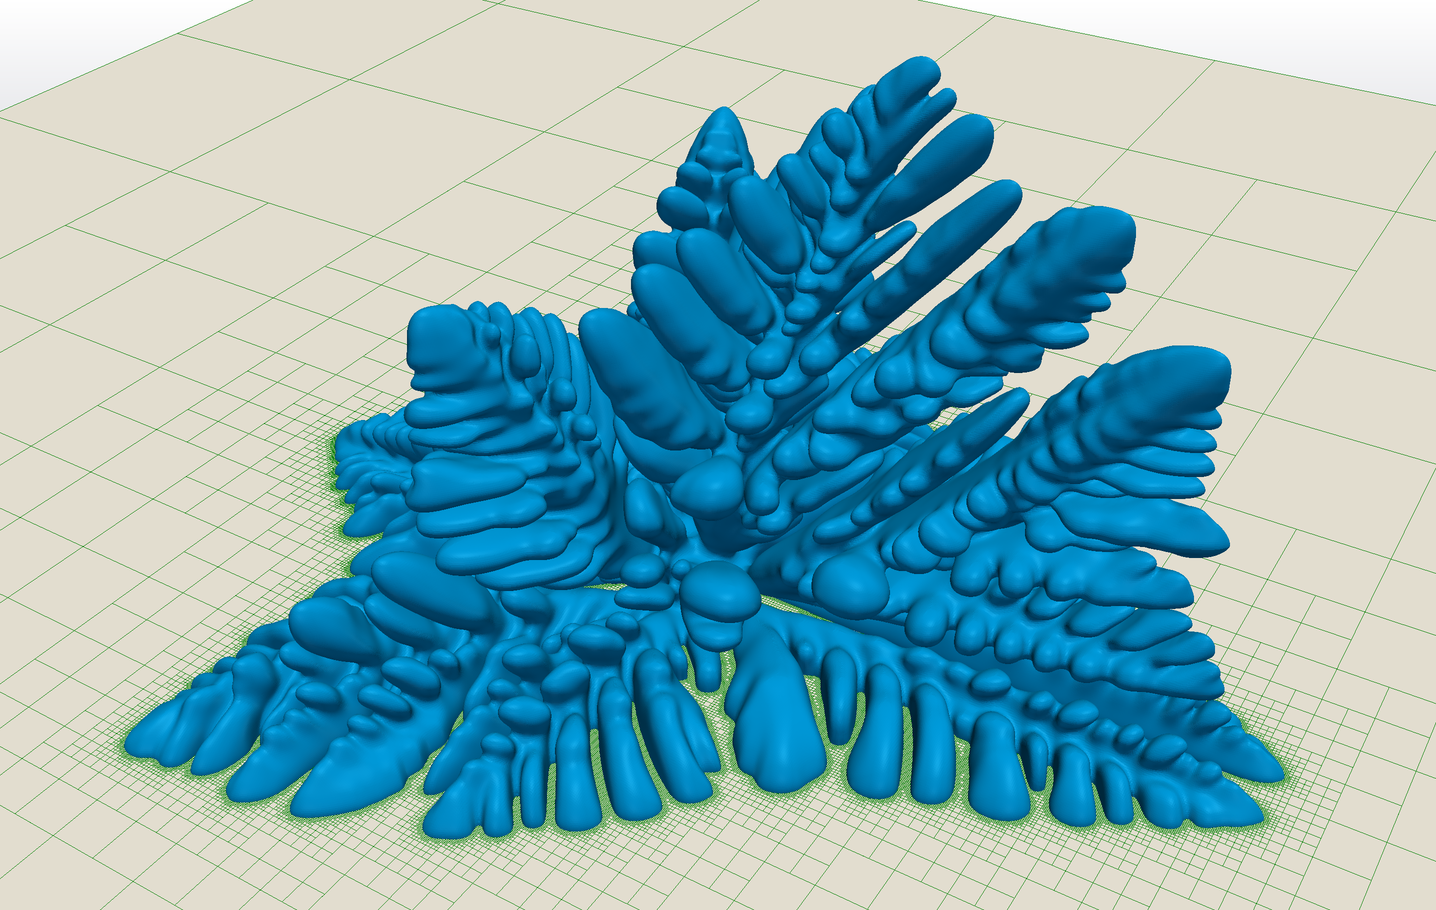
\includegraphics[width=.8\textwidth]{pictures/crystal_grid_low.png}
\end{center}
\end{figure}

\section{Acknowledgment} 

\newpage
\bibliographystyle{plain}
\addcontentsline{toc}{section}{\refname}\bibliography{references}

\end{document}